\documentclass[12pt]{article}

\title{Data Analysis Project Report}
\author{James Hughes}

\usepackage[nottoc,numbib]{tocbibind}
\usepackage{graphicx}
\usepackage[export]{adjustbox}
\usepackage[a4paper, top=13mm, bottom=19mm]{geometry}
\usepackage{url}
\usepackage[hidelinks]{hyperref}
\usepackage[labelfont=bf]{caption}


\newcommand\NA{\mathit{NA}}

\begin{document}

\begin{titlepage}
    \begin{center}
        \vspace*{5cm}

        \Huge
        \textbf{Structured Illumination Microscopy Image Processing using Deep Learning}

        \vspace{0.5cm}
        \LARGE

        James Hughes

        Supervised by Dr Edward Ward

        \vspace{2cm}
        \Huge
        \textbf{Project Report}

        \vfill

        MPhil, Data Intensive Science

        \vspace{0.8cm}

        \Large
        Department of Physics \& Department of Chemical Engineering and Biotechnology

        University of Cambridge

        United Kingdom

        28th June 2024

        (Word count: 6596)

    \end{center}
\end{titlepage}

\pagenumbering{roman}

\newpage
\section*{Acknowledgements}
\addcontentsline{toc}{section}{\protect\numberline{}Acknowledgements}

Firstly I would like to thank my supervisor, Dr Edward Ward, for all of his support over the course of this project.
Having trained originally in mathematics as an undergraduate,
the project involved a lot of concepts from microscopy and image processing that were very new to me,
but Dr Ward was quick to provide reading materials and support to help me to become more familiar with the subject matter.
He has consistently been an enthusiastic supervisor and was always there to answer any questions I had.
The chance to go into the laboratory and capture real microscope images that were later used in the work was incredibly exciting.
Dr Ward was eager to provide this opportunity and welcomed me to the Chemical Engineering and Biotechnology (CEB) Department and his research group.

I also had the opportunity to attend some of the Laser Analytics Group (LAG) lab meetings,
where I had the privilege of learning about some of the world-leading research being undertaken by the group.
Later, I shared details about the project in two presentations to the group.
I would like to thank all of the members of LAG for welcoming me, listening to my presentations and providing great feedback.
In particular I wish to thank Professor Clemens Kaminski for his helpful suggestions and words of encouragement during these meetings.

I would also like to thank Jeremy Wilkinson, Esther Gray, and Emilio Luz-Ricca.
I had helpful discussions with all of them about the findings of the project and the challenges involved,
and these conversations opened up insightful dialogues that helped me to learn more about their work,
and the nature of scientific research in general.

Lastly, I would like to thank my parents for being a continual source of support and strength throughout my education,
in particular for encouraging me to make the most of every opportunity that has come my way.

\newpage
\begin{abstract}
    \addcontentsline{toc}{section}{\protect\numberline{}Abstract}

    Structured illumination microscopy (SIM) produces images whose resolution exceeds the Abbe diffraction limit imposed on widefield images.
    However, continuous SIM imaging of dynamic cellular processes is restricted by the effects of phototoxicity, which limit the maximum duration of such time-lapses.
    In 2023, Li et al. developed a `two-step denoising' approach to SIM image processing,
    enabling a reduction in illumination intensities of the microscope,
    and in turn using deep learning to mitigate resulting noise and artefacts in the reconstructed image.
    Firstly, this project presents a data processing pipeline which implements their method using PyTorch.
    This pipeline is documented, modular, and open-source, enabling researchers to apply the method to different datasets, or develop extensions to the work.
    Secondly, this project investigates the reproducibility of this method, by analysing its performance on two datasets:
    endoplasmic reticulum and microtubule images acquired using a 2D SIM microscope and
    synthetic 3D SIM images simulated by using data from the Visible Human Project as ground-truth.
    Results indicate that although the first-step reconstructions can improve the fidelity compared to the low signal-to-noise ratio (SNR) inputs,
    this is potentially dependent on the variety of the biological structures present in the training data.
    Moreover, while the full two-step denoising method is capable of producing images close to ground-truth according to peak signal-to-noise ratio (PSNR) and structural similarity index measure (SSIM),
    and with noticeably reduced reconstruction artefacts compared to the raw and first-step reconstructions,
    this work finds evidence that the second step is prone to omission and distortion of true structures in the image.

\end{abstract}

\newpage
\tableofcontents

\newpage
\pagenumbering{arabic}
\section{Introduction}

Fluorescence microscopy is an essential tool for microbiologists,
enabling them to view complex biological phenomena unfolding at the sub-cellular level.
Fluorescent dyes are attached to specific targets,
which then release photons in response to illumination from a laser at a suitable wavelength,
producing images that highlight specific structures of interest to researchers.
As a type of optical microscopy, the resolution of these systems is limited by the effects of diffraction.
This limit was quantified by Abbe \cite{abbe} in 1873 as a minimal resolvable distance between two points,

\[d=\frac{\lambda}{2\NA}\]

where $\lambda$ refers to the emission wavelength, and $\NA$ refers to the numerical aperture,
a property of the optical system and the imaging medium.
This resolution limit is described by the optical transfer function $O(\vec{k})$ of the microscope,
which describes the set of spatial frequencies of the sample structure that can be captured by the optical system,
and to what extent they are attenuated in the resulting image (in frequency space).
Axial resolution of optical microscopes is typically much worse than their lateral resolution.
This fact is evidenced by the optical transfer function's omission of most k-vectors that lie along and near to the z-axis,
a phenomenon referred to as the `missing-cone problem'.
This is further compounded in practice with issues such as spherical abberation.
This represents a serious obstacle to researchers attempting to view cell dynamics in greater detail.

Structured Illumination Microscopy (SIM) is a technique that combines a specialised microscope set-up,
alongside computational processing of the acquired images,
in order to surpass the classical Abbe diffraction limit.
The theoretical foundations of the technique were first established at the end of the 1990's \cite{SIM2000},
but since then there have been a range of improvements made to the technique \cite{simalgorithms}, \cite{simreview}.
While SIM does not necessarily provide the greatest improvements in resolution compared to other super-resolution methods such as STED,
it has other advantages for researchers interested specifically in capturing images of dynamic biological processes over extended periods.
This relates primarily to the issue of phototoxicity effects.
Among other mechanisms, the repeated imaging causes fluorescent material to release reactive oxygen species,
which in turn have the ability to damage components of the cell and alter otherwise healthy cellular processes \cite{phototoxicity}.
This is particularly troublesome when one wishes to view dynamic processes in live cells,
because the very process of imaging has an effect on the process being captured,
thereby limiting the duration of images that can be obtained that is faithful to the true process.
SIM offers a trade-off between resolution improvements and low photo-toxicity effects.

The paper by Li et al. \cite{keypaper} explores augmenting the SIM image processing pipeline with deep-learning techniques to improve this trade-off.
Their research explores multiple ways in which hardware and computation can be used to improve the resolution of SIM imaging.
This project investigates their `two-step denoising method'.
In this method, the illumination intensity of the SIM system is set to around 10 times lower than usual,
in order to mitigate the effects of phototoxicity.
In turn, they train two networks to denoise the acquired and reconstructed images,
in order to compensate for the noise introduced by the low illumination dose and reclaim lost image resolution.

This project aims to present a full pipeline that implements their method.
The tools developed in the repository aim to make this software accessible to other research groups looking to apply it to their own data,
with minimal work required for set-up, and compatibility with common tools used for SIM image processing.
Moreover, by adopting an open-source ethos, this project should enable the pipeline to be extended upon easily.
The second main objective of this work is to study the reproducibility of the results claimed in the original research.
In particular, Li et al. assert that this method:
\begin{itemize}
    \item mitigates the presence of artefacts in the reconstructions of low signal-to-noise ratio (SNR) acquisitions,
    \item increases the fidelity of reconstructed images by up to 3.6 dB (PSNR) on average \cite{keypaper}.
\end{itemize}
This work sets out to apply the method both to images acquired using a 2D SIM system,
as well as synthetically generated 3D SIM data, and compare the resulting reconstructions.

\section{Methods}

\subsection{SIM Reconstruction process}

Structured Illumination Microscopy stands in contrast to the conventional approach of using a uniform illumination to produce a micrograph image.
Instead, SIM microscopes usually employ a spatial light modulator (SLM) to produce a striped illumination pattern,
whose spacing is close to the Abbe diffraction limit of resolution.
When the light illuminates the sample causing it to fluoresce,
the excitation pattern's spatial frequencies interfere with the high spatial frequencies of the structures in the sample,
causing information to be exposed as lower frequency features in the resulting image \cite{SIM2008}.
Figure \ref{fig:moire} demonstrates this effect with Moir\'{e} fringes,
an interference pattern with lower spatial frequency than the two patterns that generate it.

\begin{figure}[hbtp]
    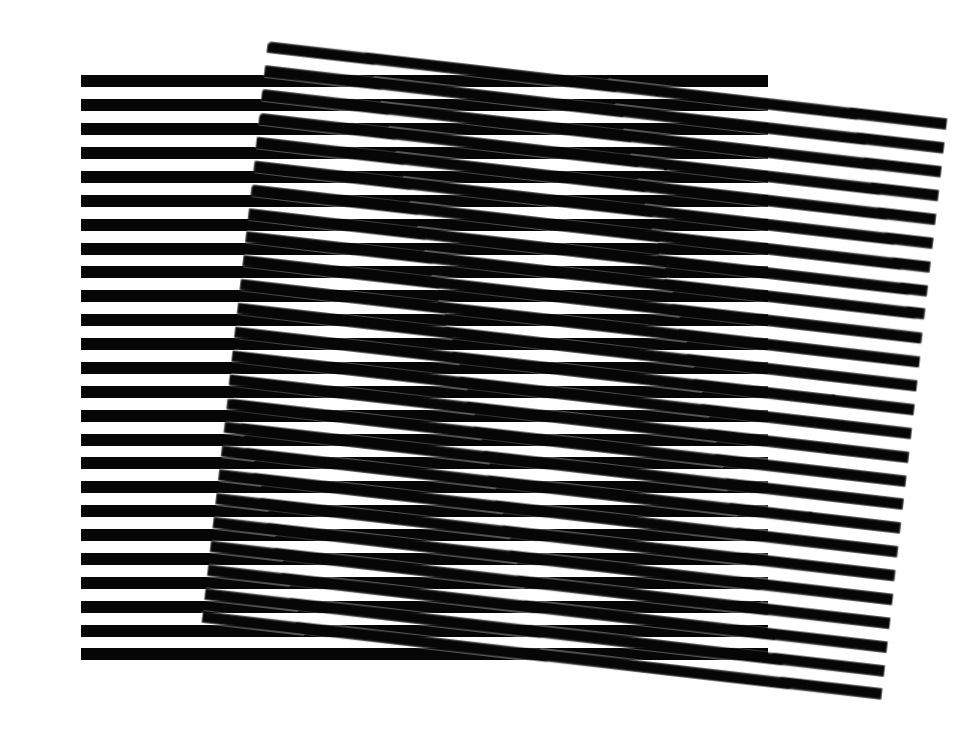
\includegraphics[scale=0.5, center]{figures/moire.png}
    \caption{\textbf{Moir\'{e} Fringes}}
    \label{fig:moire}
\end{figure}

In order to correctly interpret this interference effect, and reconstruct a super-resolved image,
multiple images need to be acquired from the microscope and analysed in the Fourier domain \cite{SIM2008}.
When reconstructed properly, there will be an improvement of lateral resolution in the direction of the k-vector of the pattern.
Therefore, when acquiring 2D or 3D SIM images, it is almost always 3 groups of images that are acquired,
using patterns with orientations at multiples of $2\pi/3$ radians,
to obtain a near-isotropic improvement in \textit{lateral} resolution (see Figure \ref{fig:SIM_otf}c).
Within these groups, the images are acquired with the illumination pattern having a different phase each time,
typically with a constant offset between phases.

The reconstruction involves six key steps:

\begin{enumerate}
    \item parameter estimation,
    \item fourier transform,
    \item band separation,
    \item Wiener filtering,
    \item apodization, and,
    \item inverse Fourier transform.
\end{enumerate}

Parameter estimation is primarily concerned with the position of the illumination pattern,
including the phase, angle, and modulation depth.
This is more accurate than measuring these quantities in the physical system which would require a high degree of care and precision to be a viable method.
The images are then passed through a Fourier transform,
since this linearises the equation to be solved during band separation.

Denoting the image intensity by $D(\vec{r})$, the pattern k-vector and phase by $\vec{p}$, $\phi_n$,
the modulation depth by $a_m$, the density of the fluorescent substance as $S(\vec{r})$ and the point-spread function (PSF) by $H(\vec{r})$,
we see that the effect of the optical system on the `true' ground-truth structure $S$ is to multiply it with the excitation pattern,
and then convolve with the point-spread function \cite{SIM2008}:

\[D_n(\vec{r}) = \sum_{m=-M}^{M}{S(\vec{r})a_m\exp(im(2\pi\vec{p}\cdot\vec{r}+\phi_n))\otimes H(\vec{r})}.\]

Utilising the Convolution Theorem \cite{convthm} this becomes

\[\tilde{D}_n(\vec{k}) = \sum_{m=-M}^{M}{\exp(im\phi_n)a_m\tilde{S}(\vec{k}-m\vec{p})\tilde{O}(\vec{k})},\]

with $\tilde{O}(\vec{k})$ representing the optical transfer function (OTF), the Fourier transform of the PSF.
In turn, with sufficiently many images acquired at different phases, namely M, this constitutes a fully determined set of linear equations for the terms:

\[\tilde{S}(\vec{k}-m\vec{p})\tilde{O}(\vec{k})\qquad m=-M,\dots,M-1,M\]

Solving this set of equations is referred to as band separation \cite{SIM2008},
and explains why 2D SIM uses 3 sets of 3 images, while 3D SIM uses 3 sets of 5 images;
the number of different phases used in imaging must correspond to the number of delta peaks that represent the illumination pattern in Fourier space,
in order to set up a fully-determined system of linear equations \cite{params}.

Whereas a conventional widefield image takes the form $\tilde{S}(\vec{k})\tilde{O}(\vec{k})$ in the Fourier domain,
so that the maximum observable spatial frequencies are determined by the radius of the OTF---the Abbe limit---
the result of this band separation is a \textit{collection} of functions in which even higher spatial frequencies have been modulated into this observable range.
The final steps therefore involve synthesising this information to produce an image with super-resolution.
Figure \ref{fig:SIM_otf} shows how the spatial frequency content of the super-resolved image compares to that of a widefield image.
The steps of Wiener filtering and apodization are used to achieve this objective,
whilst also mitigating the production of common artefacts from this combination of bands,
such as ringing and hammerstroke noise \cite{params}.
The parameters used for the reconstructions are shown in Table \ref{tab:reconparams}
---these were chosen primarily to match the physical (or simulated system),
and in the case of parameters relating to artefact reduction (such as the Wiener parameter),
these were chosen in line with best practices as suggested by \cite{params}.
Crucially, within each image class, the same parameters were used to reconstruct the high SNR, low SNR, and step 1 images.

\begin{figure}[hbtp]
    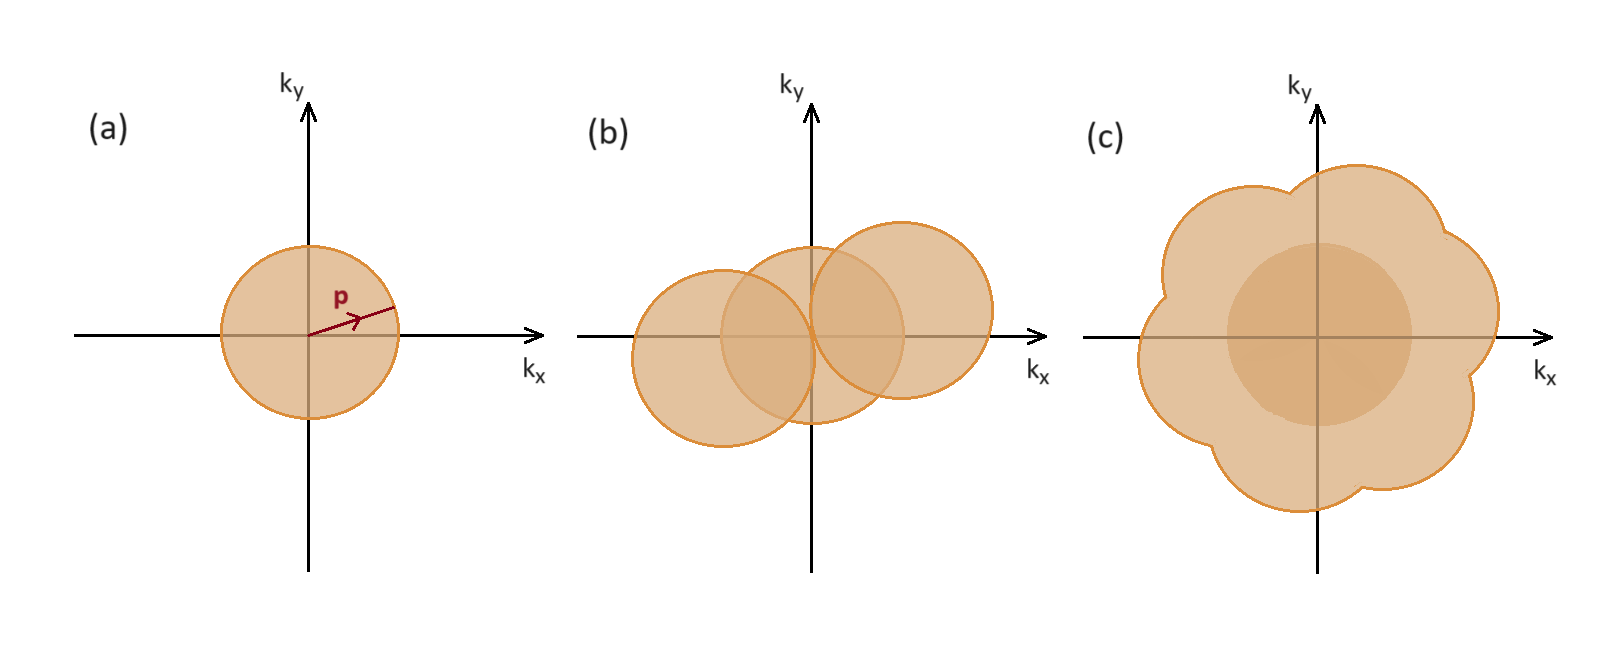
\includegraphics[scale=0.45, center]{figures/SIM_otf.png}
    \caption{\textbf{SIM reconstruction increases the range of spatial frequencies that are captured in the image.}
    (a) 2D Support of widefield OTF, with k-vector of SIM pattern, $\vec{p}$, shown.
    (b) SIM doubles the range of spatial frequencies parallel to the pattern k-vector.
    (c) Acquiring three sets of SIM images achieves near-isotropic resolution improvements laterally.}
    \label{fig:SIM_otf}
\end{figure}


\subsection{Data}

In the original work, Li et al. trained the first denoising model with pairs of high and low SNR images from a 3D SIM system,
by acquiring the same image twice using an approximately 10-fold difference in illumination intensity \cite{keypaper}.
This project used a slightly different approach,
simulating the increased image noise from using a lower illumination intensity in silico.
This made the acquisition of the training data much faster,
and avoided the need for image pair registration, along with the errors that this could induce.
A low SNR image was simulated from the ground-truth high SNR image on a pixel-by-pixel basis:
a pixel whose value is $N$ in the high SNR image was set to a random draw of a Poisson random variable with rate parameter $N$/$s$,
where $s$ was some chosen scale factor that was constant across all pixels and images.
In both datasets this scale factor was set to 20.

The method was applied to a dataset of 2D SIM images in the first instance,
in which human cells were stained with AlexaFluor 488 and ATTO 565 fluorescent dyes.
These dyes attached to the endoplasmic reticulum (ER) and microtubules, respectively.
There were 192 images in total with 96 of each type.
Earlier in the project, images from a sample in which the cell membrane and viruses infecting the cell were highlighted,
but the high spatial frequency content in the ER and microtubule images was found to be better suited to investigating the super-resolution performance of SIM and of the two-step method.
The sample was illuminated with visible light at 488nm and 561nmm.
Figure \ref{fig:2DSIM} shows just one SIM acquisition of each of the two targets,
demonstrating the appearance of the fine structured illumination.

\begin{figure}[hbtp]
    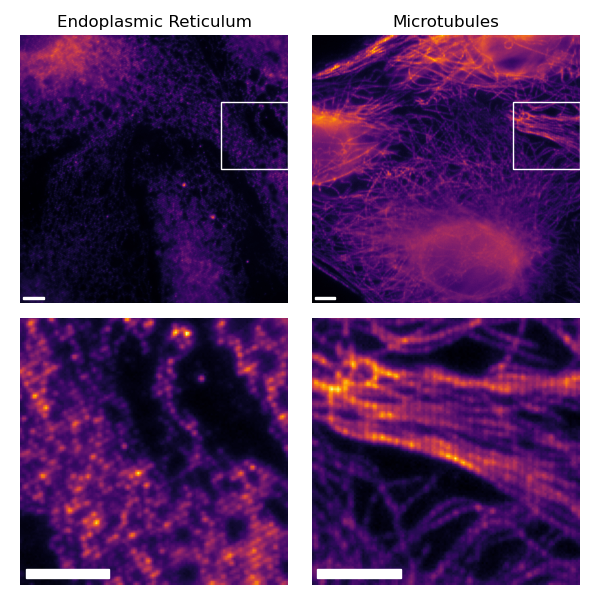
\includegraphics[scale=0.53, center]{figures/2DSIM.png}
    \caption{\textbf{Structured illumination is visible in SIM acqusition images.}
    Top row: full-view widefield image. Bottom row: cropped region of one of 9 acquired images---the structured illumination pattern is visible.
    Scale bars are 2.1\textmu m.}
    \label{fig:2DSIM}
\end{figure}

Later, the Visible Human Dataset\footnote{Courtesy of the U.S. National Library of Medicine} was used to generate synthetically acquired 3D SIM micrographs.
This dataset was released in 1994 and provides images of human cadavers prepared as a series of thousands of thin cross sections \cite{vhdata}.
This project used the 70mm photographs of the female body dataset, specifically images 2000 through to 2383.
While these images do not capture \textit{microscopic} biological structures,
those biological structures present are complex enough to yield a reasonable approximation to the kinds image features one might expect from a typical SIM micrograph of a cell.
These images were downloaded, cropped into 256x256 squares and stacked into image volumes of size 128x256x256.
Figure \ref{fig:vhcrop} shows the lateral cropping scheme overlayed onto image 2192.
The cropping is designed to produce 60 image volumes that mostly overlap with the biological subject matter,
for a total of 180 volumes when all 384 images are processed.

\begin{figure}[btp]
    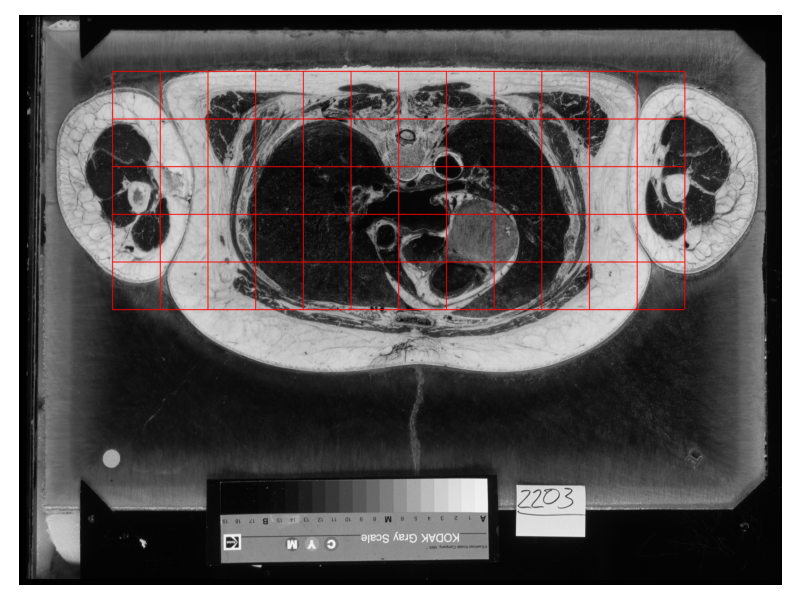
\includegraphics[scale=0.65, center]{figures/visible_human_volumes_grey.png}
    \caption{\textbf{Visible Human Project images were cropped and stacked to form synthetic image volumes.}
    Female cadaver 70mm image 2192.}
    \label{fig:vhcrop}
\end{figure}

The volumes were then processed using \texttt{generate\_sim.py} to generate synthetic SIM acquisitions.
Originally this code, provided by a previous student, took an image volume of size 64x256x256 and generated an image stack of size 15x256x256,
simulating 15 3D SIM acquisitions from a microscope whose focal plane is at the central (32nd) slice of the 3D volume.
This was adapted further to simulate a 3D SIM microscope with a vertically moving objective lens and focal plane.
This effect was achieved by cropping some of the lowest lateral slices of the 3D volume and padding the top of the volume with the same number of zero-filled layers,
in order to move the simulated focal plane upwards in the original volume.
A loop was used to generate a full 32x15x256x256 3D SIM acquisition stack,
equivalent to imaging the top half of the sample.
Each of the image volumes generated with a height of 128 voxels was used to generate two of these stacks.
Figure \ref{fig:3D_SIM} shows an example of a simulated widefield and reconstructed SIM image volume.

\begin{figure}[hbtp]
    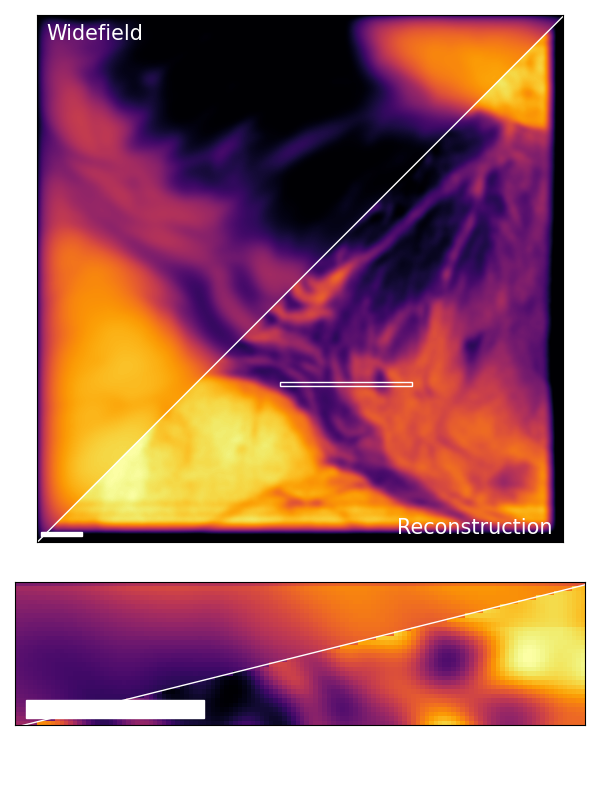
\includegraphics[scale=0.8, center]{figures/3DSIM_recon.png}
    \caption{\textbf{Super-resolution reconstruction reveals fine details hidden in widefield.}
    Top: central lateral cross-section. Bottom: Axial view from highlighted region. Scale bars are 1.0\textmu m.}
    \label{fig:3D_SIM}
\end{figure}

\subsection{Pipeline}

The first step of the data processing pipeline is the partition of training, validation, and testing datasets,
which can be done using the \texttt{image\_noising.py} script.
This takes a directory of high SNR images, generates their synthetic low SNR counterparts,
and then splits the data into training, validation, and testing partitions randomly.
In this work, 20\% of each dataset was reserved as testing data,
and a further 20\% of the remaining images were reserved for validation at the end of each training epoch.

An RCAN model is then trained using this partitioned data---the `first-step' model.
This step is handled by the \texttt{train.py} script.
The code first reads in the configuration for training from a JSON file.
This file specifies:
\begin{itemize}
    \item training hyperparameters; such as number of epochs and the learning rate,
    \item model hyperparameters, and,
    \item file management; including the frequency of model checkpointing and the locations of training and validation data.
\end{itemize}
Configuring the hyperparameters in this way ensures that it is easier to keep track of the many training runs that may be performed.
Next, the training and validation data is read one file at a time, to perform checks---for instance to ensure that all of the images are of the same shape,
and that the data is consistent with model hyperparameters.
After this, the relevant training objects are instantiated: the model itself, the Adam optimizer, and the learning rate scheduler.
If an intermediate model checkpoint has been provided, all of these objects are updated to match the state of this checkpoint,
to enable continued training.
Alongside these is the \texttt{SIM\_Dataset} object wrapped in a \texttt{torch.utils.data.DataLoader} which handles the batching of training (and validation) data.

During training, this dataset object handles generation of suitable ground-truth and raw data.
Crucially, the RCAN input shape is smaller than the images themselves,
so the \texttt{SIM\_Dataset} takes random matching crops of the training pairs that correspond to the RCAN input shape.
It then normalises the pixel values, using an affine rescaling to map extreme image-wide pixel value percentiles to 0 and 1;
this work uses the values 2\% and 99.9\% respectively.
Before these crops are outputted, they are also subjected to a random 90 degree rotation about the z-axis,
and two random reflections in the lateral axes.
By employing these simple transformations for data augmentation,
we ensure that the very fine illumination structure signal is not degraded by, say, pixel value interpolation,
so that the reconstruction algorithm performance is unaffected.
Accordingly, the dataset object also takes a \texttt{steps\_per\_epoch} parameter---this
parameter controls exactly how many times each image in the dataset is exposed to the training loop per epoch,
but with various different possible augmentations.
In addition, the object is also able to filter for regions of interest.
The number of pixel values (scaled in the $[0, 1]$ range) that exceed some intensity threshold can be counted,
and then crops with an insufficient fraction of pixel values above this level can be excluded.
However, this slows down the speed of batch-loading, not just because of the rejection rate,
but also the computation required to run this check.
This feature was only enabled during the training of the first-step in the 2D pipeline,
since the slow-down was too severe in all other cases.

The model is then applied to the raw images, using the same pixel standardisation as before
leaving the ground-truth, raw, and restored SIM acquisition stacks,
which are pre-processed before reconstruction.
Specifically, each image has its acquisitions equalised so that they all have equal total pixel intensity.
We then perform a background subtraction of the lowest 10\% of pixel values, as well as clipping the brightest 0.1\% of pixel values.
In both cases the extreme values are masked at the threshold percentile intensities.
The data is then scaled to full 16 bit-depth range and saved.

The SIM reconstruction algorithm is then applied to the three sets of images.
For this purpose, fairSIM 1.4.1 \cite{fairSIM} was used.
While the original authors of the work provide their own software that can perform this reconstruction,
fairSIM presents a standard, open-source tool that is widely used for SIM image processing,
therefore making it worthwhile to investigate if the method is reproducible with this specific implementation of the reconstruction.
To this end, part of the codebase is dedicated to enabling compatibility with the fairSIM application.
Namely, the scripts:
\begin{itemize}
    \item \texttt{convert\_omx\_to\_czxy.py},
    \item \texttt{convert\_omx\_to\_paz.py}, and,
    \item \texttt{manage\_stack.py},
\end{itemize}
can be used to convert between CZXY format (used for model training) and the OMX and PAZ formats.
This is particularly useful in the case of 3D image reconstructions which take much longer,
since in our case 32 reconstructions have to be performed per image.
Converting to PAZ and then stacking the SIM acquisition stacks enables the fairSIM `batch' feature to be used,
to automate the reconstruction of the entire stack.
Once the reconstructions are performed they are destacked,
if necessary, and postprocessed to clip negative values that arise in the SIM reconstruction,
and again scaled to the full 16 bit-depth range and saved.

At this point the `first-step' reconstructions, those from the restored acquisition stacks,
can be compared to the reconstructions from the low and high SNR data.
Additionally, the training data for the second-step denoising model can be collated.
This second model takes the restored reconstructions as its input, and the high SNR reconstructions as its target.
After training, the model is applied to the testing high SNR reconstructions, and post processed in the same way as previously.

It takes a long time to process the entire pipeline to develop the full two-step denoising method for a particular configuration of hyperparameters and training data.
The longest parts of the pipeline are the model training loops themselves.
In this work, every model was trained for 36 hours using an Nvidia A100 graphical processing unit.
The intermediate reconstructions using fairSIM can also take a long time to process---for the 3D SIM images in which half of the data needed to be reconstructed,
the reconstructions required about 2.5 hours of compute time\footnote{on a personal computer with an Intel\textcircled{R} Core\texttrademark i5 processor},
notwithstanding the pre-processing and post-processing this requires.
Additionally, the full generation of the synthetic 3D dataset required 18 hours of compute time in total.
In practice, this was achieved in under 2 hours, by using multiple CPU nodes of the CSD3 computing services to process the data in parallel.

In order to effectively carry out the project using both a personal computer for development,
and remote computing services for intensive computation,
it was crucial to use robust version control, data organisation, and I/O practices in order to keep track of multiple models being trained simultaneously,
and the configurations of these models.
The remote and local codebases were kept synchronised using git version control.
The model training hyperparameters were passed to the training script using a .json file,
which was then saved with an identifying model name to keep track of these parameters.
Models were also regularly saved using .pth checkpoints during training,
which saved the current state of the model weights and training parameters such as the learning rate scheduler.
In addition, the model hyperparameters were saved in these checkpoints,
so that models could easily be loaded and analysed using the utility function \texttt{rcan.utils.load\_rcan\_checkpoint}.
Moreover, the remote and local codebases were kept synchronised using git version control.
Crucially, a main and dev branch were used for the majority of the development process,
with a `release' branch being used later to take snapshots of the code at key points.
After the training of the models referred to in this report,
release version 1.0 was saved.
Release version 1.1 contains some further changes to the software,
including a unit testing suite and refactoring of the codebase for improved modularity and readability.

A number of software development practices were used to ensure that the processing pipeline was maintainable, robust and reproducible.
Maintainability was mainly achieved by writing explicit, readable code in the first instance.
The style of the code was enforced via pre-commit hooks that are triggered in each commit,
which included the application of Flake8 \cite{flake8} and Black \cite{black}---respectively a code linter and reformatter which enforce style guidance prescribed by PEP 8 \cite{pep8}.
This gave the code a consistent appearance throughout making it easier to follow.
A focus on building modular code further improved the maintainability of the software,
and also made the flow of the code easier to follow.
This was achieved primarily by creating two separate custom packages,
the main being \texttt{rcan} which is based on the \texttt{rcan} package developed in \cite{rcan2021},
and a second, \texttt{synthetic\_sim}, containing code used to convert image volumes from the Visible Human Project into synthetic 3D SIM images.
This aspect of the software meant that it was easy to make changes during the course of the project,
and means that there is scope for the software to be extended.

\subsection{RCAN}

In both instances, the denoising models were implemented using the residual channel attention network (RCAN) architecture,
which first emerged in the computer vision literature in 2018 \cite{rcan2018}.
The fundamental component of this architecture is the `channel attention layer'.
This unit:

\begin{itemize}
    \item summarises the features extracted in each hidden channel using a global pooling operation,
    \item computes attention weights for each channel via a simple mechanism;
    namely downsample the number of channels using a 1x1 convolution,
    apply ReLU activation,
    upsample to the number of original channels via 1x1 convolution,
    and apply sigmoid activation, and,
    \item multiply each channel from the input to the layer by the computed attention weights.
\end{itemize}

This instantiates a `channel attention mechanism', enabling the network to model complex relationships between features which can lead to better predictions.
The RCAN builds on this elementary component by combining multiple channel attention layers (or blocks) into 'residual groups'.
A single group consists of a series of 3x3 convolution layers to extract features,
followed by a channel attention layer, together with a residual connection in which the input is added.
Many of these layer sequences are chained together to form a single residual group.
Moreover, an RCAN itself consists of multiple residual groups chained together,
with intermediate residual connections as well as a `long' skip connection which spans the entire network length.
This complex residual structure of the network implements a model which, theoretically, is very deep.

Li et al. employed a slight variant of the RCAN implemented more recently \cite{rcan2021}.
In particular, this variant is re-implemented as a denoising model rather than a super-resolution model,
so there is no upsampling of the images over the course of the network architecture.
However, the code provided alongside this more recent work is written in TensorFlow.
In order to make the code compatible with the software available (specifically the versions of CUDA and cuDNN available) on the HPC platform used,
this codebase was migrated to PyTorch.
This also has the advantage of making the software more accessible to other researchers wishing to develop in PyTorch.

\section{Results}

\subsection{2D SIM Results}

\begin{figure}[hbtp]
    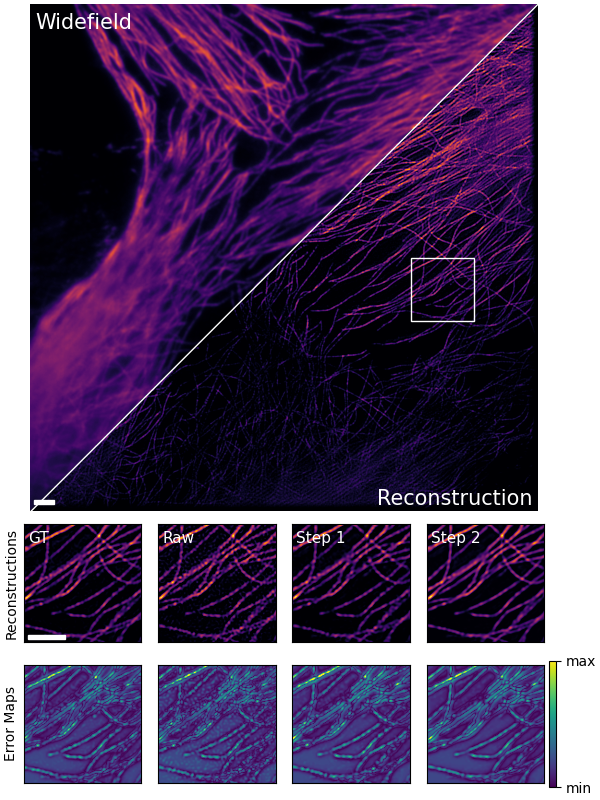
\includegraphics[scale=1.05, center]{figures/mt_1_008_error.png}
    \caption{\textbf{First and second step reconstructions removed ringing artefacts.}
    Top: Full ground-truth (GT) image. Bottom: Reconstructions and error maps from high SNR, low SNR, and restored images.
    Scale bars are 2.1\textmu m.}
    \label{fig:microtub_samples}
\end{figure}

\begin{figure}[hbt]
    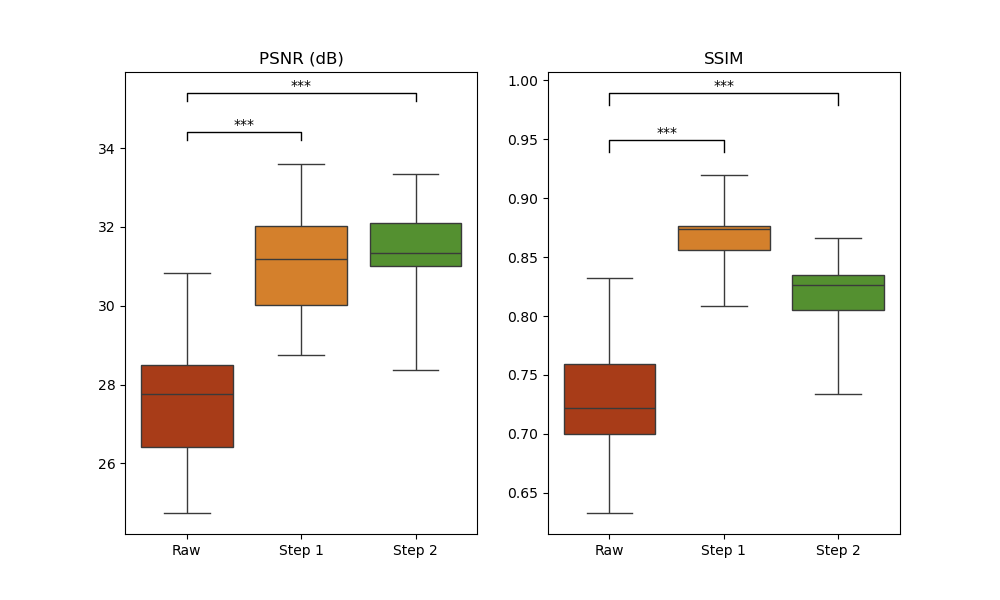
\includegraphics[scale=0.7, center]{figures/boxplot_mt_only.png}
    \caption{\textbf{Both denoising steps consistently improved PSNR and SSIM of images compared to GT.}
    Performance of pipeline trained to reconstruct microtubule images, evaluated on the test dataset (N=20).
    Asterisks denote significance of a two-sided paired t-test, using APA convention (number of stars = $-log_{10}(p)$).}
    \label{fig:m019_m020_pipeline_stats}
\end{figure}

The 2D image processing pipeline used RCAN models with a 128x128 input region,
and an architecture comprising 5 residual groups of 3 blocks each (slightly smaller than that of the 3D models).
During image denoising, the input image is patched into regions having a 32 pixel overlap,
and the model is applied to each region independently.
The predictions are then averaged in regions of the image where patches overlap,
avoiding the creation of edge artefacts at the borders of the patching regime.
The same training, validation, and testing data was used to train both networks.

Initially, only the microtubule images were used for model training.
Both models were trained for 500 epochs.
Figure \ref{fig:microtub_samples} shows an example of the denoising pipeline applied to an image from the test dataset.
In the `raw' reconstruction we can see the ringing artefacts created by the increased noise in the SIM acquisitions used.
The step 1 reconstruction was achieved by denoising the low SNR acquisition before applying the reconstruction,
while in step 2, this reconstruction was passed through the further second model.
In both of the denoised reconstructions, we observe a removal of the ringing artefacts present in the low SNR reconstruction.
Figures \ref{fig:microtub_samples}, \ref{fig:er_samples} and \ref{fig:vh_samples_error} also show `error maps' produced using the NanoJ-Squirrel plugin for ImageJ \cite{squirrel}.
These error maps compare the super-resolution images (reconstructions) to the original ground-truth widefield image,
by estimating a `resolution scaling function (RSF)', convolving this with the super-resolved image,
and plotting the difference in pixel values with the widefield image.
These error maps indicate areas in the super-resolution image that are subjected to reconstruction artefacts.
In Figure \ref{fig:microtub_samples}, the error map highlights the ringing artefacts in the background region of the low SNR reconstruction.

Figure \ref{fig:m019_m020_pipeline_stats} shows the results of applying this pipeline to the test data.
The complete two-step reconstructions have a PSNR with reference to the ground-truth reconstructions which is on average 3.8 dB higher than the low SNR reconstructions.
Similarly the SSIM improves by 0.09 on average.
These improvements correspond to a qualitative improvement in the reconstruction in Figure \ref{fig:microtub_samples}.
However, most of this improvement can be attributed to the first-step model.
Indeed, the reconstruction does not appear to change much visually after the second step denoising,
and in fact the SSIM of the reconstruction decreases by 0.05 on average after the second step is applied.
Additionally the first-step reconstructions appear to be more consistent in their quantitative improvements than the full two-step restoration.

\begin{figure}[hbtp]
    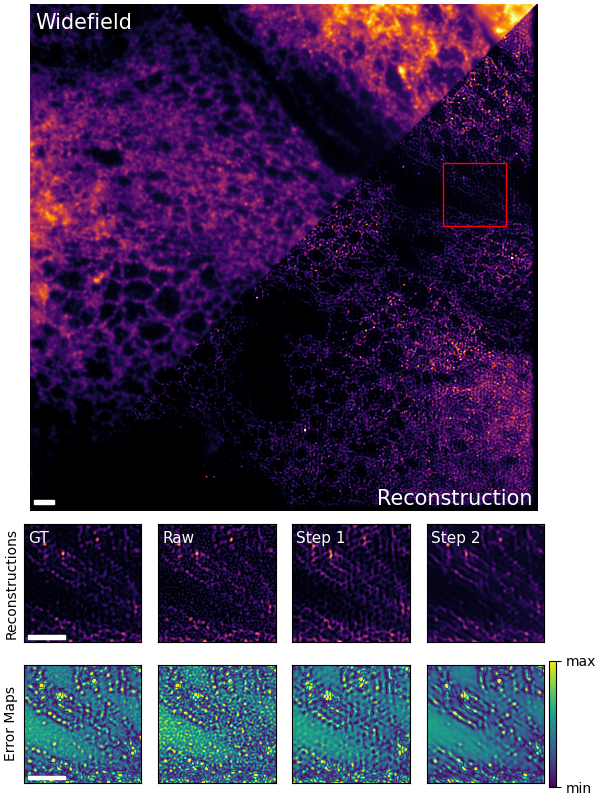
\includegraphics[scale=1.05, center]{figures/mt_0_016_error.png}
    \caption{\textbf{First step reconstructions introduce new patterned artefacts.}
    Sample of the results from the 2D SIM restoration pipeline applied to both fluorescence channels.
    Top: Full ground-truth (GT) image. Bottom: Reconstructions and error maps from high SNR, low SNR, and restored images.
    Scale bars are 2.1\textmu m.}
    \label{fig:er_samples}
\end{figure}

\begin{figure}[hbt]
    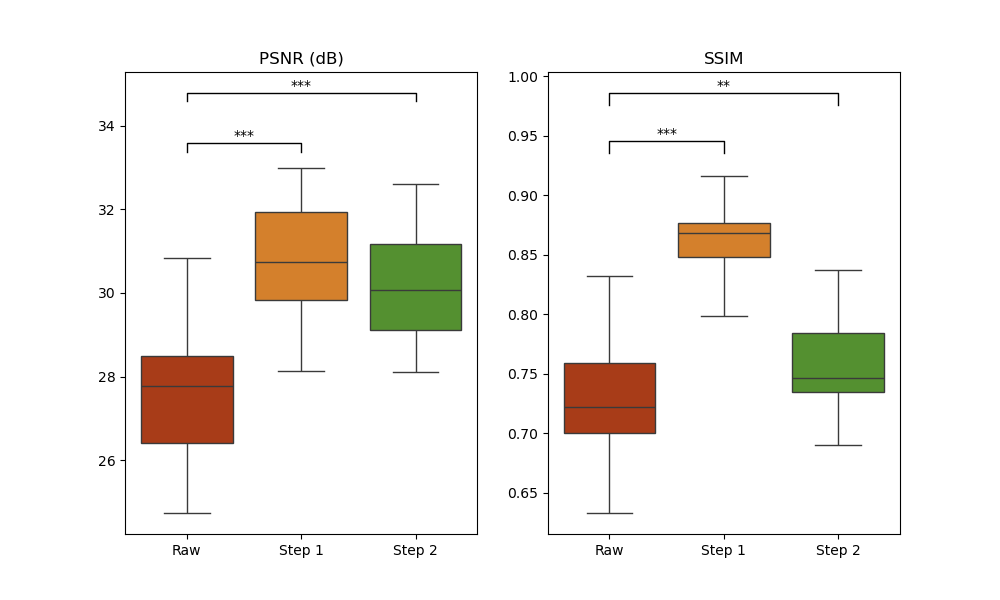
\includegraphics[scale=0.72, center]{figures/boxplot_2d_1.png}
    \caption{\textbf{Two-step reconstructions of microtubule images worsened when other images were added to the training data.}
    Performance of pipeline trained to reconstruct all 2D images, evaluated on the \textbf{microtubule} images in the test dataset (N=20).}
    \label{fig:m023_m024_561_pipeline_stats}
\end{figure}

In the second instance, a pipeline with the same model hyperparameters was developed using the full dataset for model training:
both the ER and microtubule images.
The first model was trained for 245 epochs and the second for 500 epochs.
Figure \ref{fig:er_samples} shows the result of applying this pipeline to an ER test image.
As before, the low SNR reconstruction contains ringing artefacts,
however in this case rather than being removed outright in the first-step reconstruction,
these are replaced by a different set of patterned artefacts.
These manifest as hexagonal patterns in the step 1 error map.
The full two-step reconstruction manages to mitigate these new artefacts,
although it is concerning that some of the rough textures of the ground-truth reconstruction appear to be lost in the second step.
This raises the possibility that in the denoising process,
it may be difficult for the model to discriminate between true fine features and artificial ones introduced by noise.
The inspection of restoration performance in Figure \ref{fig:er_samples} is reflected in Figure \ref{fig:m023_m024_488_pipeline_stats},
where the quantitative evaluation of both steps of this model decreases in terms of both PSNR and SSIM, for ER images.
It is worth noting that the fidelity of the low SNR ER images is higher on average than for the microtubules,
however even in absolute terms, both the first-step and two-step denoised images perform much worse than the previous restoration pipeline in terms of the SSIM metric.
Additionally, increasing the diversity of training data also worsens the performance on the microtubule images;
the two-step form of this model only provided an increase of 2.6dB in PSNR and 0.03 for SSIM,
and a similar observation is true for the first-step restoration.
In fact, some of the highlighted regions in the step 2 error map in Figure \ref{fig:er_samples} take on a similar appearance to the microtubules.
This may indicate that even the slightest diversity in the training data confuses the model---in
such a way that in this case,
the second denoising step erroneously morphs features of the ER image into features seen in the microtubule images.

\begin{figure}[hbt]
    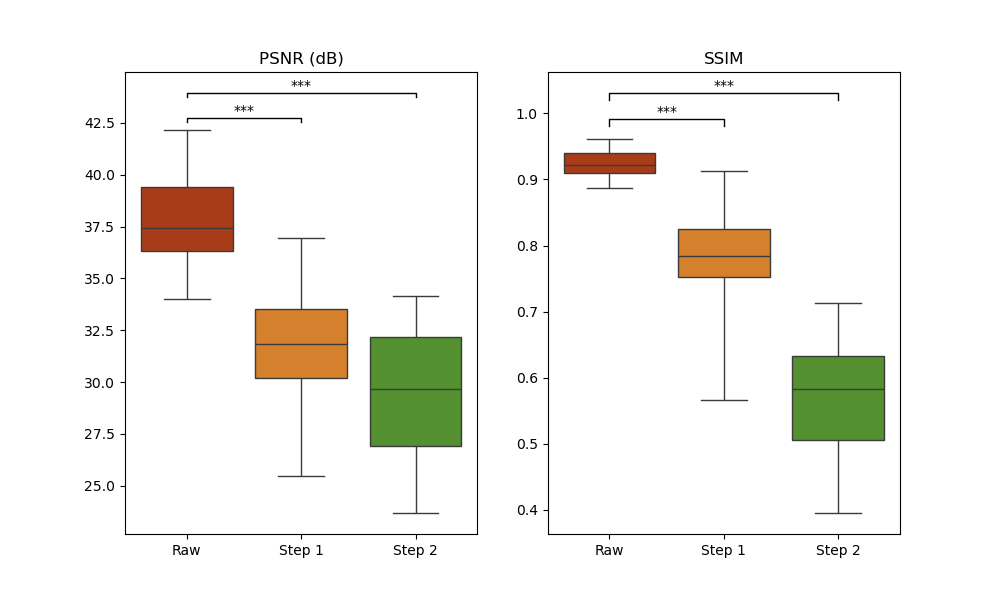
\includegraphics[scale=0.72, center]{figures/boxplot_2d_0.png}
    \caption{\textbf{Applying the two-step reconstruction to ER images caused PSNR and SSIM to decrease.}
    Performance of pipeline trained to reconstruct all 2D images, evaluated on the \textbf{ER} images in the test dataset (N=20).}
    \label{fig:m023_m024_488_pipeline_stats}
\end{figure}


\subsection{3D SIM Results}

For the 3D data, the same training hyperparameters were used, except for the architecture.
Slightly larger RCAN models with 5 residual groups of 5 blocks each were used---matching the architecture employed by Li et al.
Additionally---unlike for the previous models---for this pipeline the entire dataset was divided into two sets of 180 image volumes,
enabling separate training and validation datasets for the first model and the second model.
In order to construct these datasets for the second model, the first-step model had to be trained,
and then applied to the training data for the second step model.
This should theoretically improve the performance of the second network,
since it is being trained on reconstructions that have been produced by passing a previously unseen image into the first-step model,
which more closely matches the situation at the time of deployment of the full pipeline after training.
The drawback of this approach is that the training datasets for each network are halved in size.
The first step model was trained for 41 epochs, the second for 24.

\begin{figure}[hbtp]
    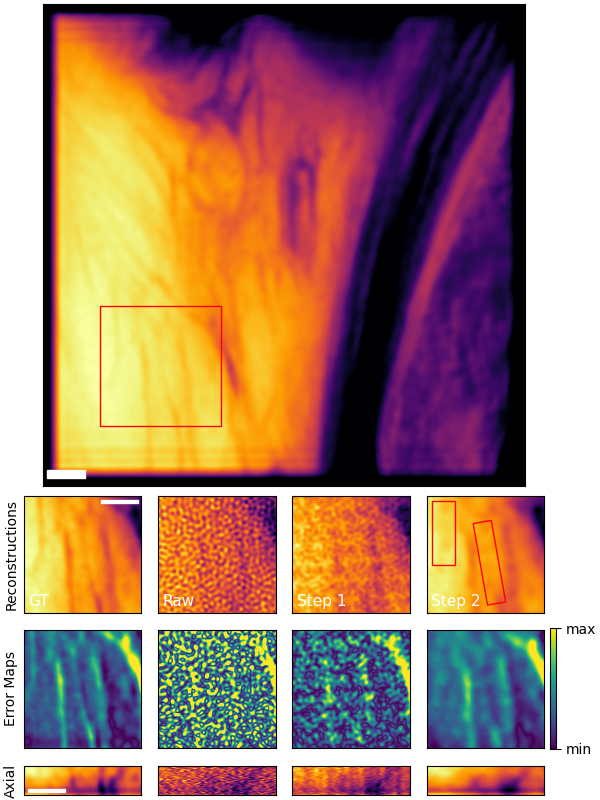
\includegraphics[scale=1.05, center]{figures/vh_error.png}
    \caption{\textbf{Sample of the results from the 3D SIM restoration pipeline.}
    Top-to-bottom: Full ground-truth (GT) image, lateral views, error maps, axial views of reconstructions.
    Red skeleton superimposed onto lateral views is fixed. Scale bars are 1.0\textmu m.}
    \label{fig:vh_samples_error}
\end{figure}

Figure \ref{fig:vh_samples_error} demonstrates an example of one of the reconstructions of the two-step model.
The low SNR reconstruction suffers from irregular ringing artefacts, similar to those seen previously in the 2D pipeline.
As before, the first-step reconstruction removes these artefacts,
but appears to introduce new patterned artefacts.
This is a common observation of the first step 3D reconstructions,
and in multiple cases in Figure \ref{fig:3D_further_samples} the first step introduces artefacts in the form of a regular triangular lattice
---this was found to be frequent around the edges of high intensity regions.
Similarly, the axial views of the first-step reconstructions appear to be affected by regular patterned artefacts in the form of vertical `stripes'.
These are somewhat visible in \ref{fig:vh_samples_error} and even more apparent in Figure \ref{fig:3D_further_samples}.

The full two-step restoration mitigates these artefacts in both the lateral and axial planes,
but appears again to be indiscriminate between features resulting from ground truth stuctures and those resulting from noise.
The step 2 reconstruction in Figure \ref{fig:vh_samples_error} shows an example of this,
with key features from the ground-truth reconstruction missing from the restored image (highlighted by the red rectangles in the latter).
This is also the case in the axial views, where key ground-truth features from the axial view appear to be `smoothed over' or distorted.
The phenomenon is highlighted by the error map for the second step.
Compared to the ground-truth error map, the errors in the step 2 map simply appear more spatially uniform.
This points to the higher PSNR and SSIM scores of the two-step reconstruction being achieved by removing patterned noise artefacts,
but also sometimes via a loss or distortion of true structures in the images.
This can be seen in some of the images in Figure \ref{fig:3D_further_samples},
for instance the two-step reconstruction in the top row which has an SSIM of 0.95 compared to ground-truth,
yet clearly has lost some of the fine textures of the ground-truth reconstruction.

\begin{figure}[htb]
    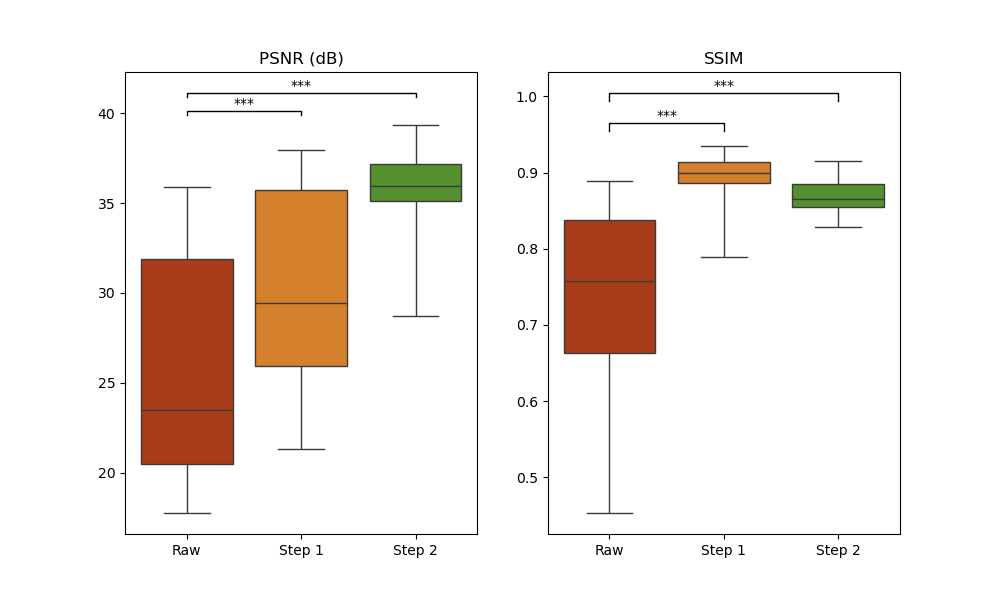
\includegraphics[scale=0.75, center]{figures/boxplot_3d.png}
    \caption{\textbf{Two-step reconstructions of 3D image volumes caused PSNR to increase by 9.8 dB, and SSIM by 0.13, on average.}
    Performance of pipeline trained to reconstruct Visible Human images, evaluated on the test dataset (N=36).}
    \label{fig:vh_stats}
\end{figure}

Figure \ref{fig:vh_stats} shows the quantitative performance of the 3D SIM restorations.
According to both PSNR and SSIM, the 3D SIM restoration improves the data fidelity of the low SNR images quite considerably.
The two-step reconstructions lead to a 9.8\textpm 1.1 dB increase in PSNR in total,
with the first denoising step contributing 4.8\textpm 0.3 dB.
Similarly the SSIM improves by 0.13\textpm 0.02 as a result of the full two-step restoration,
although in this case the second step appears to slightly degrade the first-step reconstruction.
For comparison, the original work found that in a sample of 11 images of immunolabeled Tomm20 in fixed U2OS cells,
the two-step method led to improvements of 3.6 dB in PSNR and 0.15 in SSIM, compared to the low SNR reconstructions on average \cite{keypaper}.

\section{Discussion}

This project investigated the reproducibility of the original research by Li et al. by applying the method they developed to multiple new datasets.
The sets of data used here represent different domains of images,
firstly because of the different ground-truth structures---ER and Visible Human images---and secondly
by using images acquired by SIM systems with slightly different specifications.
In particular the real images were acquired from a 2D SIM system rather than a 3D SIM system,
and even the 3D images were acquired from an optical system simulated in silico.
In the same vein, the reconstructions were performed using a more widespread tool, fairSIM,
rather than the bespoke reconstruction code used in the project,
in order to investigate whether the specific reconstruction algorithm might affect the performance of the method.
The work corroborated multiple claims that Li et al. made about the two-step RCAN method.
Indeed, this project demonstrated that the method is capable of removing ringing artefacts that result from reconstructing a stack of SIM images acquired at a low illumination intensity.
Although the first-step model can introduce new, patterned artefacts, these are typically mitigated by the further second step,
just as is observed in Figure 5c in \cite{keypaper}.
Moreover, for the microtubule-only and Visible Human denoising pipelines,
it was shown that their two-step method is capable of consistent improvements in the fidelity of the SIM image reconstruction,
according to PSNR and SSIM, across both lateral and axial views.

The work also uncovered some underlying issues with the method.
Primarily, it was shown that the absence of artefacts in the restored image,
and even a large improvement in the fidelity of the reconstruction in terms of common image comparison metrics,
are not sufficient to guarantee that the method generates a SIM reconstruction that is faithful to the ground-truth image.
The two-step denoising method was shown to consistently remove structures and change textures present in the ground-truth reconstruction.
This raises concerns over the validity of the method in the context of live-cell imaging,
since it could morph the appearance of biological structures unpredictably.
Indeed, while the method preserves the analytical reconstruction in the intermediate step,
this unpredictable behaviour of the resoration reflects the use of two very deep neural networks in the image processing pipeline
(a further `isotropization' network is used in the original work \cite{keypaper}),
compounding the pre-existing issue of the lack of interpretability of each individual model.
Moreover, the unpredictable nature of the RCAN models poses a risk to the behaviour of the analytic reconstruction,
because even small changes in the illumination pattern of the original low SNR input may lead to drastic changes in the reconstruction.
SIM microscopy relies on a precise alignment of the structured illumination,
whose exact spatial location is already being estimated during reconstruction,
and the compounding of errors in this estimation by deep-learning appears to manifest in newer artefacts introduced by the first-step reconstruction.
This means that even the role of the intermediate reconstruction in the method---the more interpretable part of the pipeline---also becomes less transparent.

Additionally, the work showed that the method is not suited to application to a diverse image dataset.
Introducing new image samples into the training data did not enable the restoration to successfully reconstruct images of that type,
and moreover degraded the performance of the method for previously included samples.
Hence, it appears that the method must be trained to reconstruct images of a single specific type of biological structure.
This raises further questions about the underlying predictions made by the denoising models.
Li et al. describe their approach as, ``embedding information about the sample into a series of neural networks''\cite{keypaper},
but this strategy may suffer from worsened performance when unexpected structures arise in the ground-truth during inference.
Indeed, much of the point of super-resolution microscopy is to observe new structures and cell dynamics,
which demands a super-resolution method that can generalize properly.

Thirdly, the work demonstrates that developing the method is highly time-consuming.
This is partly due to the large amount of data that needs to be acquired to train the RCAN models.
While the earlier approach in the 2D SIM reconstruction was to use the same training and validation data for both models,
using two separate splits of data was found to improve model performance in the 3D SIM models,
particularly in the second step.
However this contributes to a need for even more training data being acquired.
This project successfully demonstrated how the training data acquisition time could be reduced by around a factor of at least 2,
by simulating the low dose illumination imaging in silico.
The model training, as well as the reconstruction of images in fairSIM,
also takes a long time, and this is something that could be considered in future work.
One possibility is transfer learning, an approach that has already been applied to SIM reconstruction pipelines employing deep learning \cite{mlsim}
This could involve developing the foundational model on the Visible Human dataset,
and then fine tuning to a specific sample type depending on the application required.
The advantage of this approach would be that most of the training data would be synthesised completely in silico,
reducing the time and efforts of the data acqusition,
whilst meeting the requirement for the pipeline to be fine-tuned to the specific sample being imaged at the inference stage.

An iterative approach was taken in building the software for this project.
Development began with prototyping the code, starting with the key elements of the training loop and model,
which had to be migrated from the original source which was written using TensorFlow.
Models were first trained using the 2D SIM images,
which enabled the generation of some results more quickly than starting with the 3D pipeline,
whilst also verifying that key elements of both processing pipeline were working properly.
It was also helpful to learn more about the SIM reconstruction process during this time,
before developing the more involved 3D SIM denoising method.
On reflection, some of the practices applied to the software later in the project could have been considered sooner.
Indeed, in the process of generating the full documentation for the software,
some bugs were found in the code, in some instances meaning that parts of the pipeline had to be run again.
In addition, unit testing was only included in version 1.1 of the code,
and while the key aspects of the software did not change dramatically between versions 1.0 and 1.1,
this testing suite does not verify the exact software used to develop the pipelines analysed here.
Finally, the extent to which the simulated aspects of the data generation faithfully recreate realistic SIM images remains unclear.
In particular, the ground-truth SIM images generated from the Visibile Human image volumes represent an `ideal' simulation,
that does not capture some of the problems encountered during physical microscopy such as spherical aberration or illumination pattern misalignment.
The results gained from both sets of data shed new light onto the viability of the proposed method,
and the developed software could easily be used to investigate the performance of the method on another 3D SIM dataset acquired from a physical system.

\newpage

\bibliographystyle{IEEEtran}
\bibliography{Biblio}

\newpage

\appendix

\section{Reconstruction Parameters}

\begin{table}[htp]
    \centering
    \begin{tabular}{| c | c | c | c |}
        \hline
        Parameter & 2D Dataset (1) & 2D Dataset (2) & 3D Dataset \\
        \hline
        $\NA$  & 1.1 & 1.1 & 1.12 \\
        \hline
        Pixel width (nm) & 107 & 107 & 50 \\
        \hline
        Wavelength (nm) & 488 & 561 & 464 \\
        \hline
        OTF param.  & 0.15 & 0.15 & 0.15 \\
        \hline
        APO cutoff & 1.59 & 1.68 & 1.82 \\
        \hline
        APO bend  & 1.0 & 1.0 & 1.0 \\
        \hline
        Wiener parameter & 0.05 & 0.05 & 0.05 \\
        \hline
        RL Iterations & 5 & 5 & 5\\
        \hline

    \end{tabular}
    \caption{Parameters used to reconstruct the images in fairSIM \cite{fairSIM}.}
    \label{tab:reconparams}
\end{table}

\newpage

\section{Further Samples From the Two-Step Denoising Pipelines}

\begin{figure}[hbtp]
    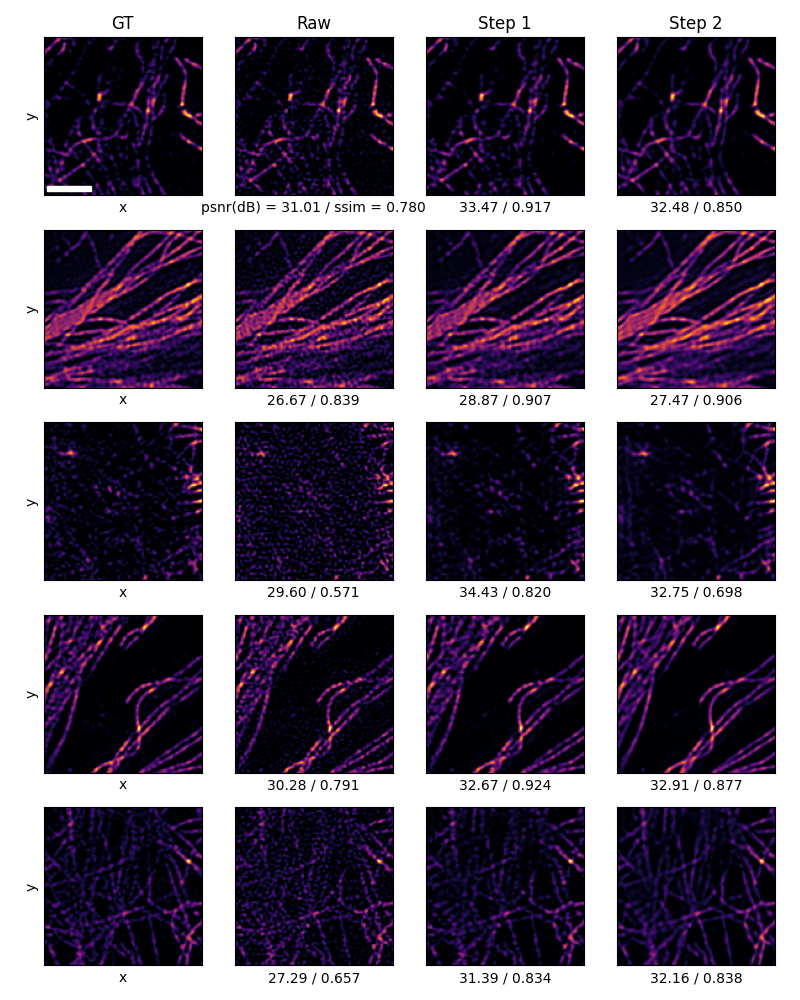
\includegraphics[scale=0.75, center]{figures/m019_m020_reconstruction_samples.png}
    \caption{Crops from a sample of 2D SIM (microtubule only) restorations compared to the low SNR and high SNR reconstructions.
    Scale bar is 1.9\textmu m.}
    \label{fig:2D_mo_further_samples}
\end{figure}

\begin{figure}[hbtp]
    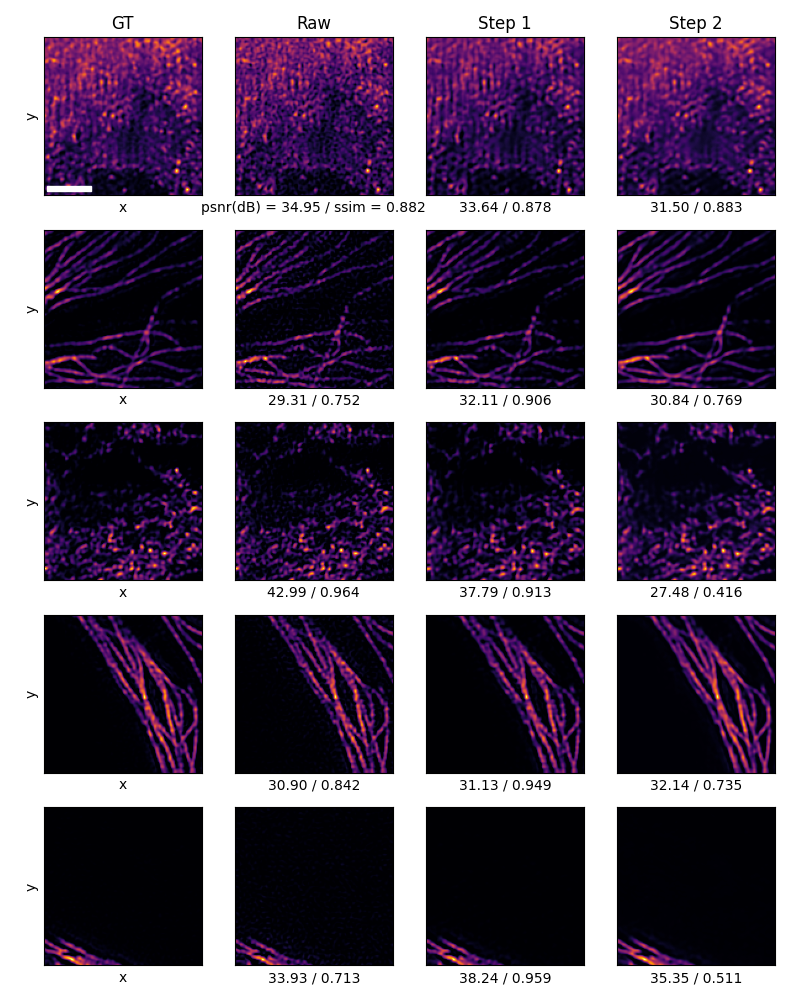
\includegraphics[scale=0.8, center]{figures/m023_m024_reconstruction_samples.png}
    \caption{Crops from a sample of 2D SIM (all data) restorations compared to the low SNR and high SNR reconstructions.
    Scale bar is 1.9\textmu m.}
    \label{fig:2D_further_samples}
\end{figure}


\begin{figure}[hbtp]
    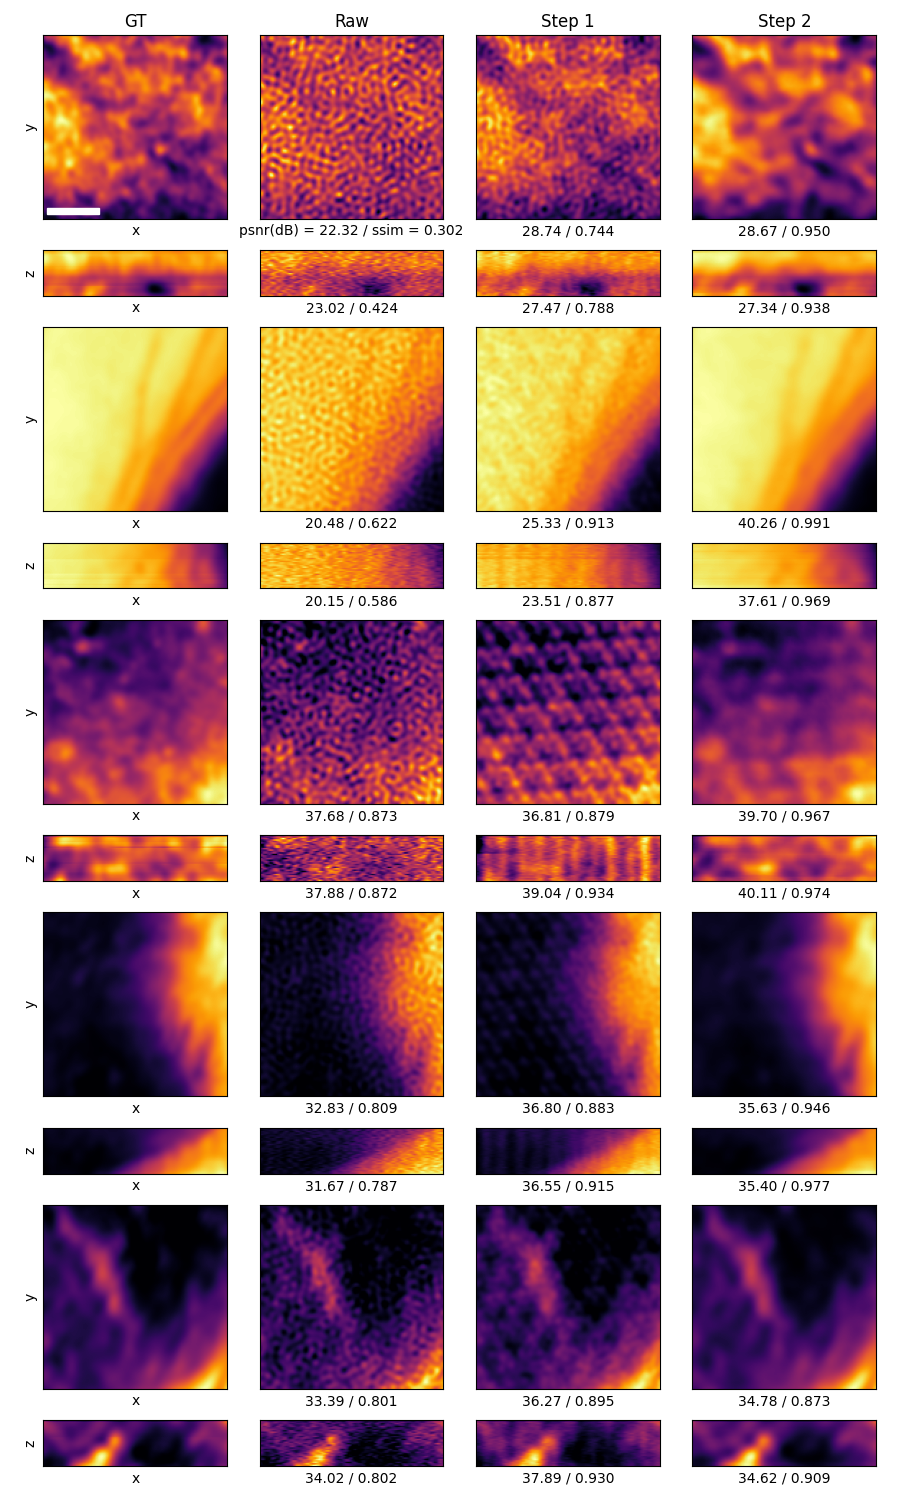
\includegraphics[scale=0.65, center]{figures/m021_m022_reconstruction_samples.png}
    \caption{Crops from a sample of 3D SIM restorations compared to the low SNR and high SNR reconstructions.
    Scale bar is 0.9\textmu m.}
    \label{fig:3D_further_samples}
\end{figure}

\newpage

\section{Statement on the use of auto-generation tools}

Auto-generation tools, such as GitHub Copilot or Microsoft Copilot, were not used at any stage during the development of the code within the repository of this project.
Similarly, none of the content of this report was produced -- or proofread -- by modern Large Language Models such as ChatGPT at any point.

\section {High-Performance Computing Resources}

This work was performed using resources provided by the Cambridge Service for Data Driven Discovery (CSD3) operated by the University of Cambridge Research Computing Service (www.csd3.cam.ac.uk),
provided by Dell EMC and Intel using Tier-2 funding from the Engineering and Physical Sciences Research Council (capital grant EP/T022159/1),
and DiRAC funding from the Science and Technology Facilities Council (www.dirac.ac.uk).

\end{document}
